\RequirePackage{amsthm} %https://tex.stackexchange.com/questions/687324/unknown-theoremstyle-warning-with-springer-nature-template
\documentclass[sn-mathphys-num,icol]{sn-jnl}
%\documentclass[sn-mathphys-num,iicol]{jnl}

%\usepackage{sn-jnl.sty}
\usepackage[pscoord]{eso-pic}% The zero point of the coordinate systemis the lower left corner of the page (the default).

\usepackage[absolute,overlay]{textpos}
\usepackage[dvipsnames]{xcolor}
\usepackage{tikz}
\usepackage{graphicx}% \usepackage{multirow}% \usepackage{cuted}
\usepackage{amsmath,amssymb,amsfonts}%
\usepackage{multicol}
\usepackage{multirow}
\usepackage{amsthm}%
\usepackage{gensymb}
\usepackage{physics}
\usepackage[locale=US]{siunitx}
\usepackage{mathrsfs}%
\usepackage[title]{appendix}%
\usepackage{xcolor}%
\usepackage{textcomp}%
\usepackage{manyfoot}%
\usepackage{booktabs}%
\usepackage{algorithm}%
\usepackage{algorithmicx}%
\usepackage{algpseudocode}%
\usepackage{listings}%
\usepackage{newtxmath}%
\usepackage{yfonts}
\usepackage{braket}
\usepackage{dsfont}
\usepackage{subfig}
\usepackage[tiny]{titlesec}%
\usepackage[american]{babel}
\usepackage{cleveref}

\usetikzlibrary{arrows.meta, positioning, shapes.geometric, decorations.markings}

\theoremstyle{thmstyleone}
\newtheorem{theorem}{Theorem}
\newtheorem{proposition}[theorem]{Proposition}

\theoremstyle{thmstyletwo}
\newtheorem{remark}{Remark}

\theoremstyle{thmstylethree}
\newtheorem{definition}{Definition}

\raggedbottom

\newcommand{\td}{\text{d}}

\titleformat{\subsection}{}{\thesubsection}{1em}{\itshape}
\titleformat{\subsubsection}{}{\thesubsubsection}{1em}{\itshape}

\begin{document}

\title{A248: MOT}
\author*[1]{\fnm{Dhruv} \sur{Pisharody}}\email{s36drohi@uni-bonn.de}
\author*[1]{\fnm{Angelo} \sur{Brade}}\email{s72abrad@uni-bonn.de}
\affil*[1]{Rheinische Friedrich--Wilhelms--Universität, Bonn}
\maketitle

\section{Abstract}
A given magneto optical trap is adjusted to trap and cool an ensemble of Rubidium atoms to a fraction of a Kelvin.
% TODO: More 

\section{Theory}
When atoms absorb photons with frequency $f$, here with a $5S_{1/2}, F=3\rightarrow 5P_{3/2}, F'=4$ transition (see \Cref{fig:scheeme}), they receive a momentum exchange of $p=\hbar f$. By detuning the Laser via a red-shift, the moving atoms slow down since the Doppler-shift blue-shifts the photons. Thus the photons only are absorbed if the atom is moving. Having two counter-propagating lasers slows their velocity in that axis. Adding two more counter-propagating laser pairs in the other axes, stops them nearly completely and thus cool them down.

Since the excited states also relax spontaneously into states like $F=2$ too, they need to be repumped by a second laser, since in this dark state the original cooling laser can not hit the $F=2\rightarrow F'=3$ frequency.

Also, through drift, they can still escape the volume. Therefor a magnetic quadrupole is created. It shifts the energy transitions through the Zeeman effect. Since it is linearly increasing with distance from the center, the transitions of atoms further away from the center are more blue shifted, i.e. the red-shifted lasers are closer to the transition frequency. Thus the atoms experience more force and are pushed to the center again.

Through temperature change or fluctuations in the electric current, the lasers can deviate from their frequencies. To counteract this, changes in the intensity of the spectra of atoms, done with the lasers, are fed back into the laser as an error-signal. Thus when the intensity changes, i.e. the laser frequency deviates, the frequency is adjusted again.

The spectrum is obtained by polarization spectroscopy. It solves the main problem, that the spectrum is Doppler broadened, since the Rubidium gas in the laser stabilization part is not cooled. For this a pumping beam is used that depletes the ground states of the atoms and a test beam is used that also passes the gas. The test beam is afterwards measured. If an atom moves away from both beam axis with the same velocity, no beam is blue shifted, i.e. they hit the same frequency. Then the test beam is not absorbed, since all ground states are depleted. The other atoms, with the same velocity, can only let the test beam pass if by coincidence the blue shift lets both, pumping and test beam, hit a transition. Since they will be different transitions, there will be more so-called cossover peaks. The polarization of the beams are discussed the \textit{Laser Stabilization} section.
\begin{figure}
	\begin{center}
		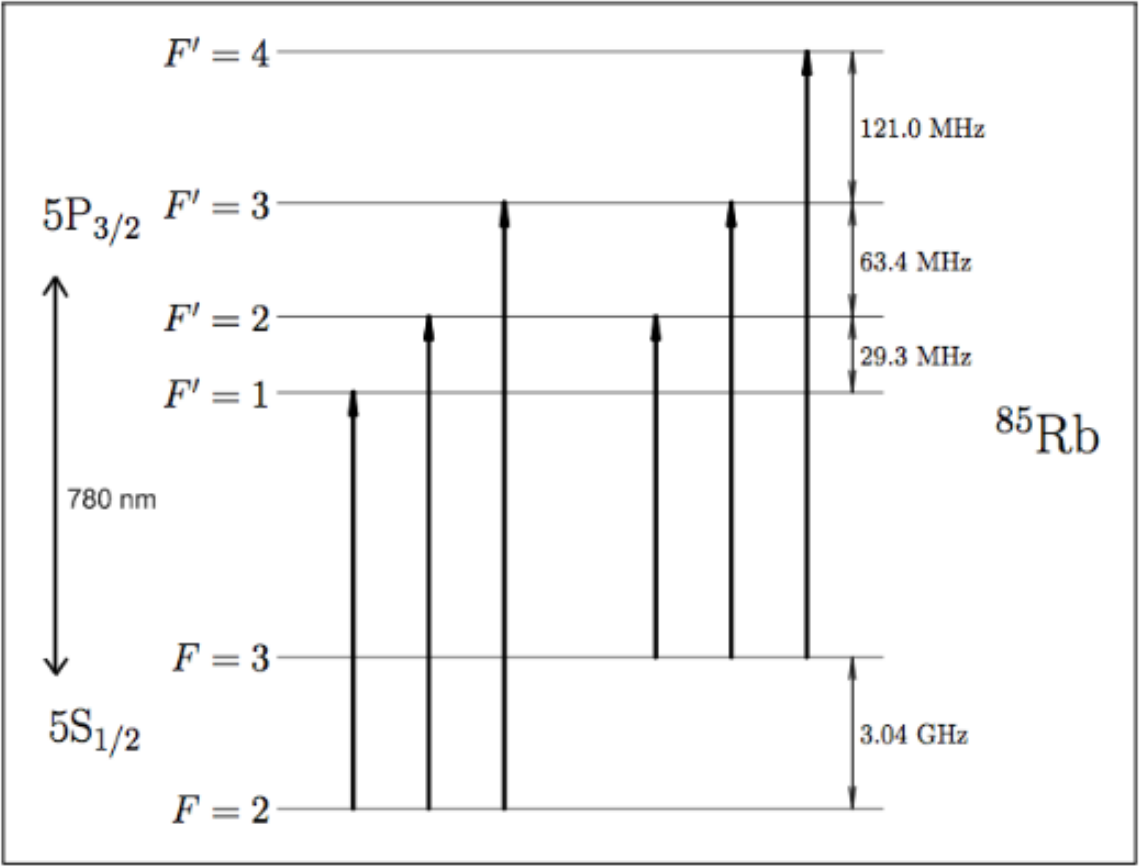
\includegraphics[width=1\textwidth]{../images/scheem.png}
	\end{center}
	\caption{Level structure of $^{85}Rb$ with cooling transition $3\rightarrow4$ and repumping transition $2\rightarrow3$.\cite{manuel}}\label{fig:scheeme}
\end{figure}

\section{Setup}
The setup consists of a laser part where the lasers are locked to the transition frequency for cooling and repumping and the main MOT part where three counterpropagating lasers cool and trap the atoms through the Zeeman shift of the magnetic field from coils in an anti-Helmholz configuration (see \Cref{fig:lp}).

\subsection{Laser}
The lasers are a cavity with a diode (DI) in the back and a reflexive window in the front, mounted on a piezo-crystal (PZ). The length determines the frequency of the escaping photons. The frequency is further filtered by an angle depended frequency filter (FI). Two lenses (LC and L2) are used to cumulate the lasers and another lens (L1) is used to reduce the laser width when it passes the PZ. See \Cref{fig:laser}

\begin{figure}
	\begin{center}
		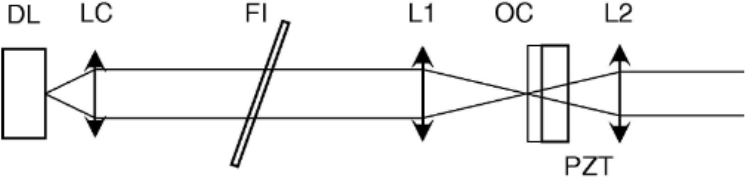
\includegraphics[width=1\textwidth]{../images/laser.png}
	\end{center}
	\caption{The Cavity constituding the Laser.\cite{manuel}}\label{fig:laser}
\end{figure}

\subsection{Laser Stabilization}
In the laser part, two lasers are set to the transition frequency for cooling ($3\rightarrow4$) and repumping ($2\rightarrow3$). They both pass the Faraday Isolator to stop any counter-propagating photons from entering the lasers. Next they pass a polarisation beam splitter (PBS) where they are split and linearly polarized. After they pass a glass plate, one beam for each laser system is rotated by $\pi/2$ and the other is circular polarized. As the circular polarized beam induces an anisotropic population in the degenerate states, and thus birefringence in the atoms, the linear polarized beam is rotated by the atoms. The linear polarized beam then passes another PBS which is orthogonal to the original beam before they passed the atoms. Therefore the intensity depends on the angle rotated, i.e. how resonant the laser frequency is with the transition. At the end the laser is split again and subtracted from each other. This resulting signal looks like the derivative of the Doppler-free absorption peak and is fed back to the laser into the piezo-crystal as the error signal to correct the cavity length, and thus the frequency, if any unwanted detuning through e.g. temperature change is induced.

While this correction is constantly done, the other portion of the laser of the first mentioned PBS is directed into an optical fiber, where both the repumping and the cooling laser merge and are redirected to the MOT.
\begin{figure}
	\begin{center}
		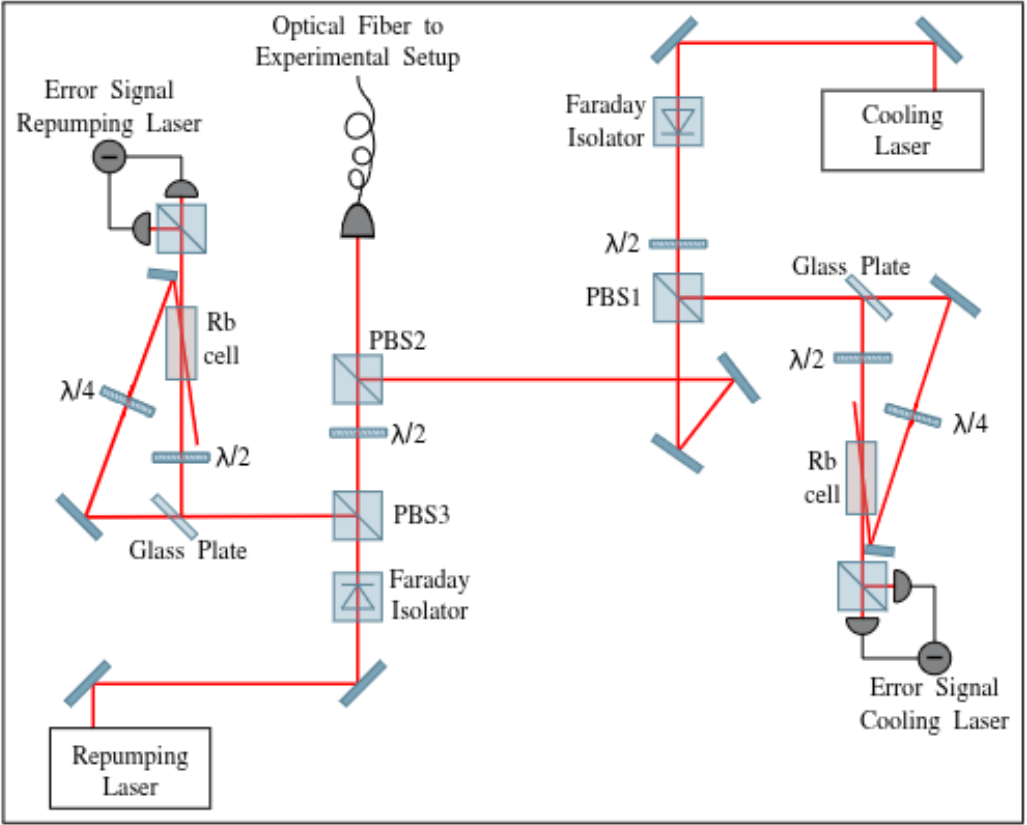
\includegraphics[width=1\textwidth]{../images/laserpart.png}
	\end{center}
	\caption{Laser part to lock the frequency to the repumping and cooling transition through polarisation spectroscopy.\cite{manuel}}\label{fig:lp}
\end{figure}
\subsection{MOT}
The actual magneto optical trap consists of two coils and the stabilized laser. The laser is split into three parts where each points in one spacial direction such that they meet at a crossing point. Further, each laser is then reflected and counter-propagated. See \Cref{fig:mot}

\begin{figure}
	\begin{center}
		
\includegraphics[width=1\textwidth]{../images/mot.png}
	\end{center}
	\caption{The MOT part.\cite{manuel}}\label{fig:mot}
\end{figure}

\section{Measurements}

% TODO

\section{Conclusion}

% TODO


\bibliography{refs}
\end{document}
